\atstartofhistorysection
\section[Un peu d’histoire : le cheval-vapeur]{Un peu d’histoire :\onlyamphibook{\\} le cheval-vapeur}
\label{ch_cheval_vapeur}

	Nous associons traditionnellement le mot \emph{moteur} à la propulsion automobile : des machines fonctionnant avec de l’air et de l’essence. Pourtant, les tout premiers moteurs étaient tout autres. Lourds, lents, incroyablement volumineux, fonctionnant au charbon et à l’eau, ils ne servaient qu’à pomper de l’eau.

	Revenons au début du \textsc{xix}\iieme siècle. À cette époque, l’Europe se chauffe au charbon, que l’on extrait à grand-peine de mines sans cesse inondées. On en retire l’eau en faisant travailler des chevaux, au travers d’un mécanisme de pompage primitif. Les premiers moteurs sont installés pour remplacer ces chevaux --\ mais ils sont à peine moins coûteux, et demandent au moins autant d’attention !
	
	\onlyamphibook{\begin{figure}[htp]}  %handmade
	\onlyframabook{\begin{figure}}
		\begin{center}
			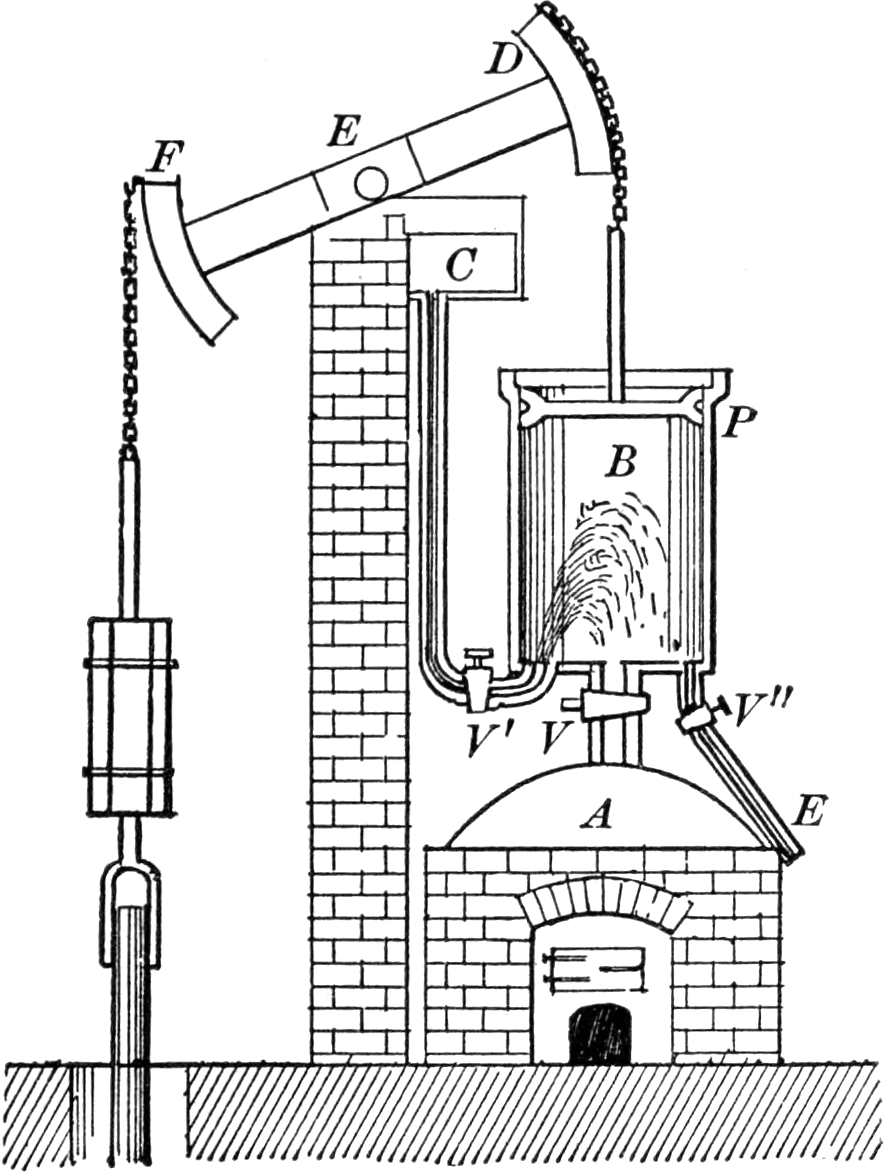
\includegraphics[width=10cm]{images/Newcomen6325.png}
			\supercaption{Schéma de coupe d’un des premiers moteurs à vapeur (moteur Newcomen, \texttildelow 1720). La condensation provoquée par injection d’eau dans le cylindre provoquait une chute de pression interne.}{\wcfile{Newcomen6325.png}{Dessin \pd par Newton Henry Black \& Harvey Nathaniel Davis}, publié en 1913}
			\label{fig_newcomen}
		\end{center}
	\end{figure}

	Les technologies métallurgique (les cylindres sont en cuivre et travaillés à la main) et mécanique (les vannes doivent être ouvertes et fermées une à une manuellement tout au long du fonctionnement), toutes deux balbutiantes, cantonnent ces moteurs à des pressions de fonctionnement très faibles.

	Pour ces moteurs, l’eau convient parfaitement. Lorsque la vapeur à pression modérée est refroidie (par exemple en y mêlant de l’eau liquide froide), elle se condense et sa pression chute brutalement (\cref{fig_newcomen}). C’est l’occasion d’entraîner un piston qui, soumis à la pression atmosphérique sur son autre face, pourra produire du travail. Ainsi, on pourrait presque parler de «~moteurs à implosion~», puisqu’ils font travailler l’atmosphère sur un cylindre de vapeur dépressurisée pour produire du travail.

	Avec ce mode de fonctionnement, la différence de pression obtenue atteint au plus \SI{1}{\bar}, et la cadence est lamentablement faible. Mais l’ensemble fonctionne à température et pressions raisonnables et les exploitants ne manquent ni de charbon, ni d’eau.

	C’est un jeune employé de l’université de Manchester qui réalise le premier le potentiel de développement formidable qui s’offre au moteur. En étudiant un modèle réduit de moteur appartenant à l’université, il apporte une série de modifications qui vont doubler son rendement.

	\begin{figure}
	\begin{center}
		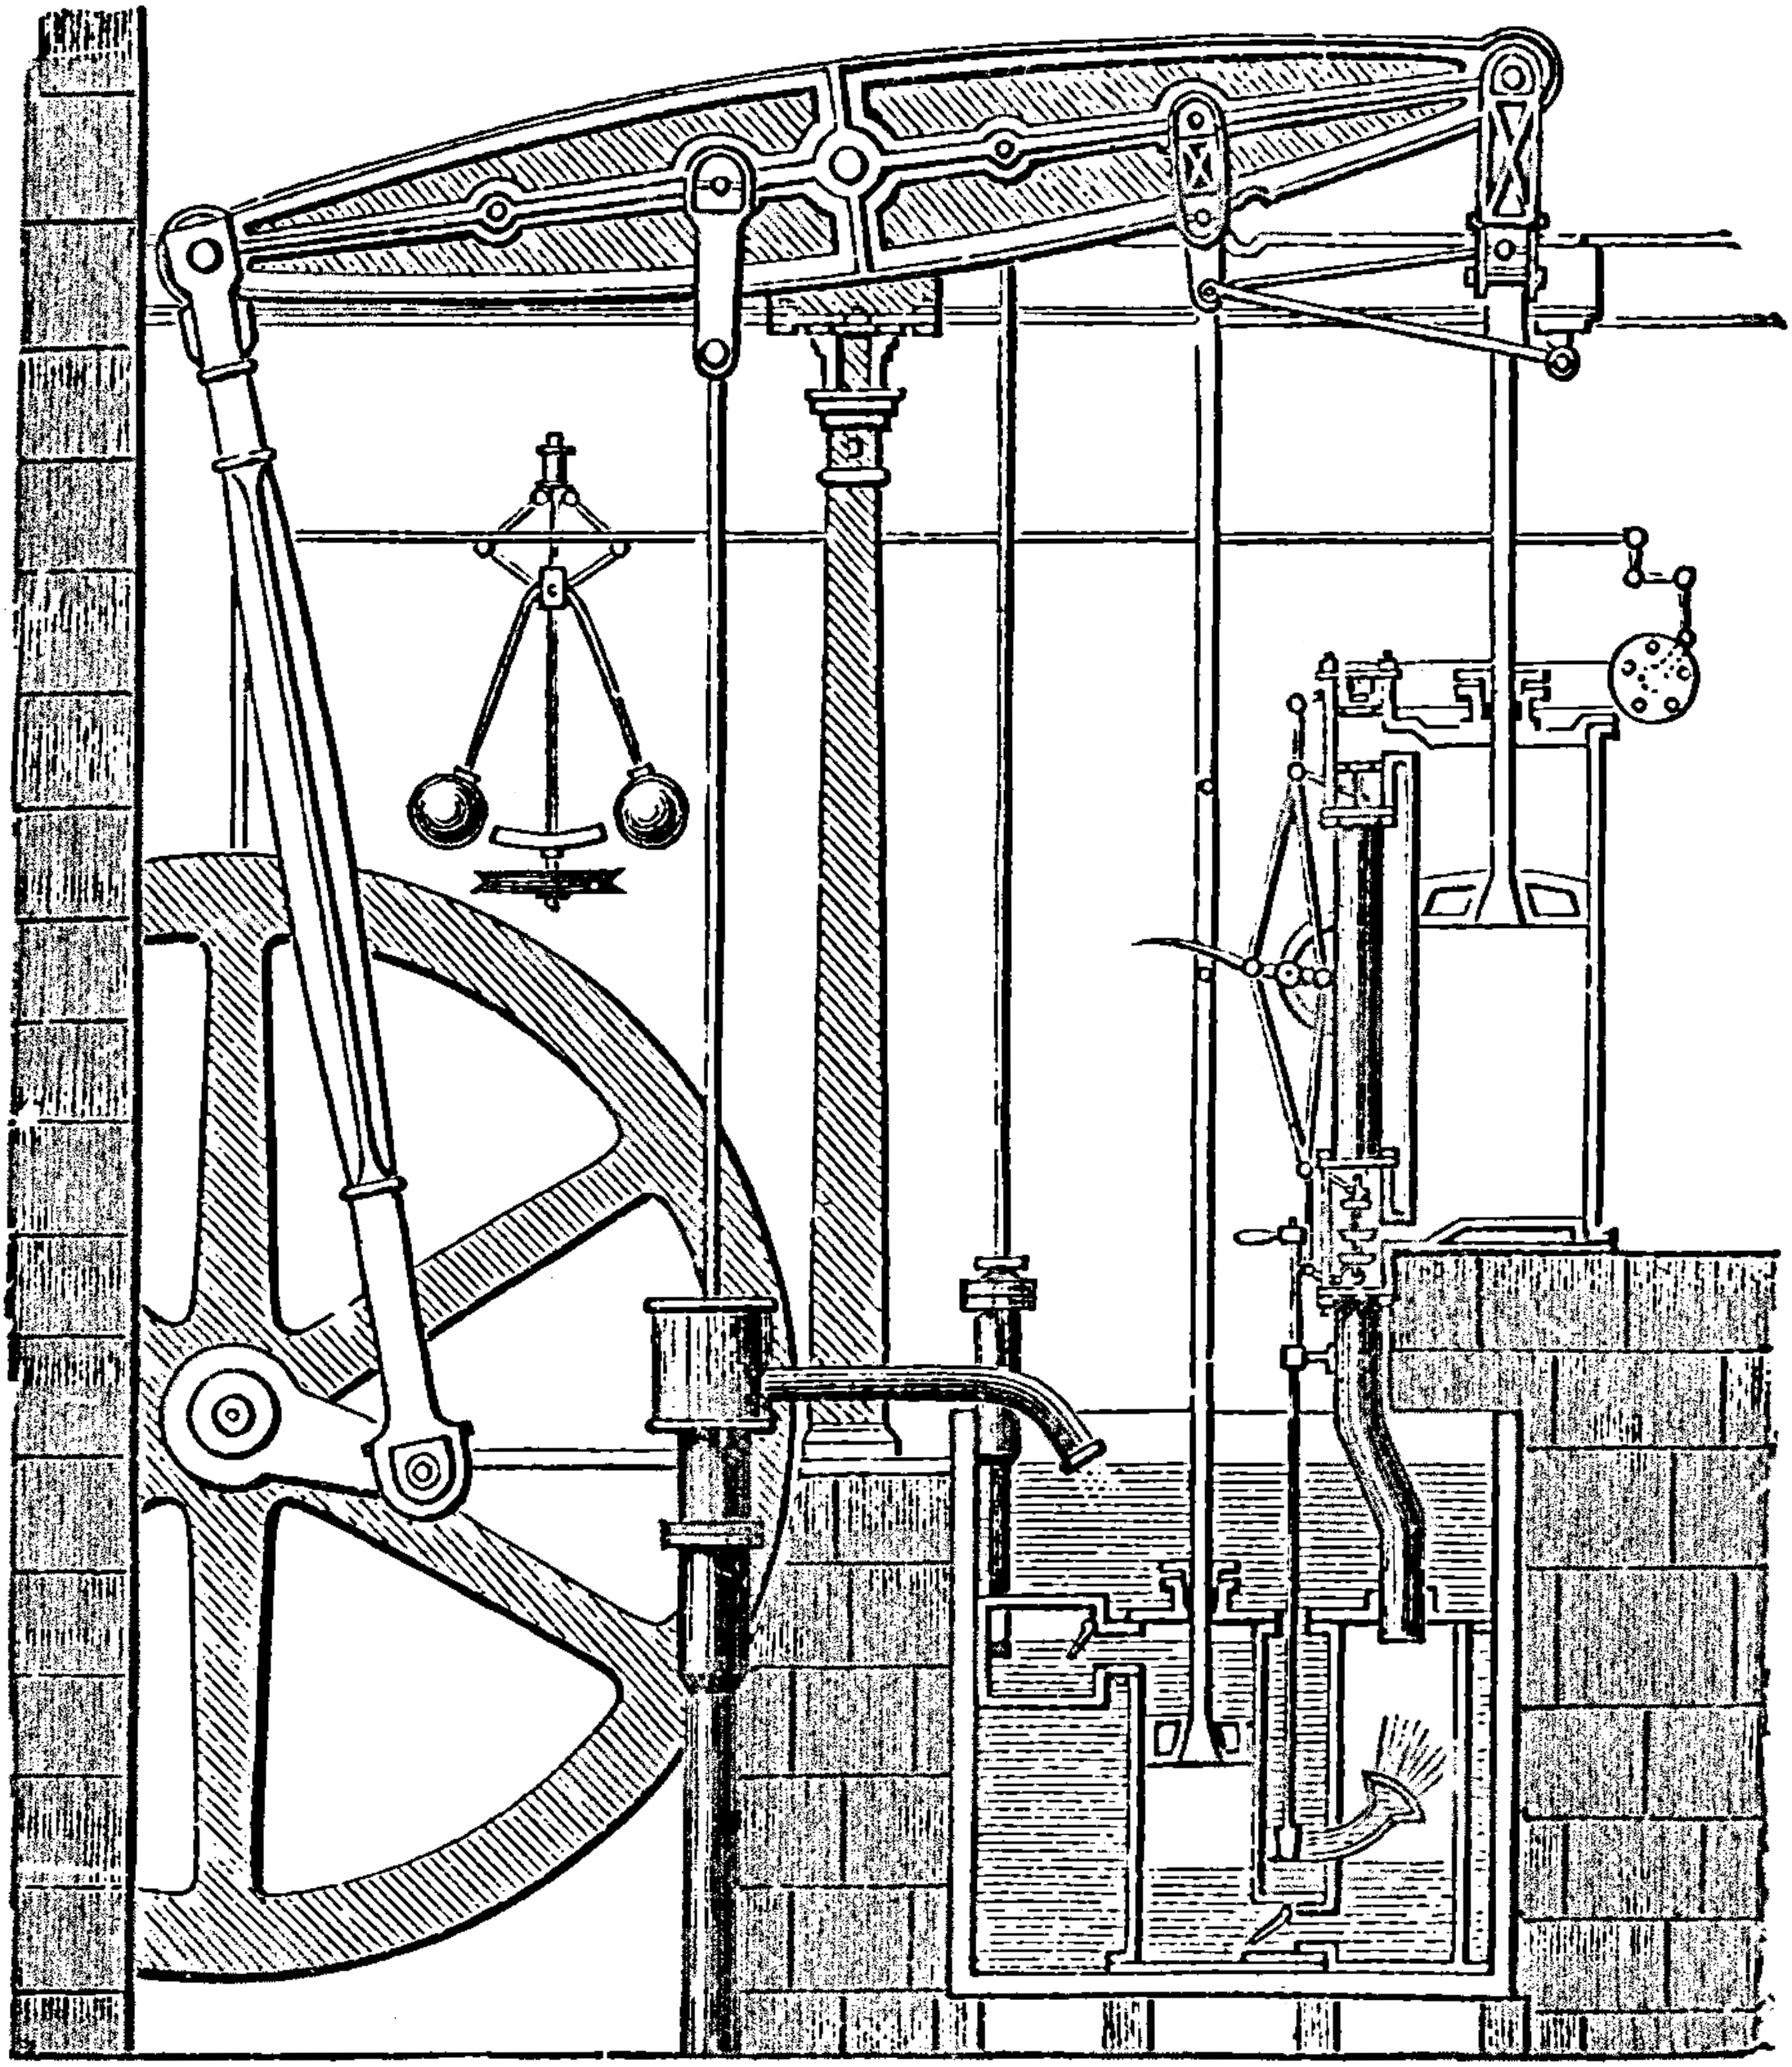
\includegraphics[width=10cm]{images/steam_engine_boulton_watt.png}
	\end{center}
	\supercaption{Le moteur de \textit{Boulton \& Watt} avec condensation séparée et piston double-face.}{\wcfile{SteamEngine_Boulton\%26Watt_1784.png}{Dessin} \pd par Robert Henry Thurston (1878)}
	\label{fig_boultonwattengine}
	\end{figure}

	La première et la plus importante de ces modifications va être de séparer dans l’espace les phases de réchauffement et de refroidissement de la vapeur. Auparavant, la condensation par injection d’eau froide abaissait aussi la température du piston et du cylindre métalliques, qu’il fallait, à chaque cycle, réchauffer, avec un coût en chaleur important. Désormais, la vapeur est refroidie dans une chambre maintenue à basse température par immersion dans l’eau (\cref{fig_boultonwattengine}), tandis que le cylindre moteur est maintenu à haute température au-dessus de la chaudière.

	La seconde modification va consister à exploiter les deux faces du piston. En utilisant un système de conduites contrôlées par des vannes, il devient possible d’augmenter la différence de pression animant le mouvement du piston. Tandis que la vapeur se condense à~\SI{0,2}{\bar} d’un côté, l’autre face subit désormais la pression de la vapeur à~\SI{1,4}{\bar}. Non seulement le travail fourni à chaque mouvement de piston est augmenté mais, en plus, la cadence (et ainsi la puissance) est doublée, puisque le piston est moteur en se déplaçant vers le haut comme vers le bas.

	Pour finir, une série d’automatismes mécaniques réduisent l’attention qu’il est nécessaire d’apporter à la formidable machinerie ainsi assemblée. Le volant d’inertie maintient la cadence, l’ouverture des vannes est mécaniquement liée à l’avancement du moteur, et le régulateur centrifuge à boules, hérité des moulins à eau et ainsi devenu célèbre, évite l’emballement ou le calage.

	\begin{figure}
	\begin{center}
		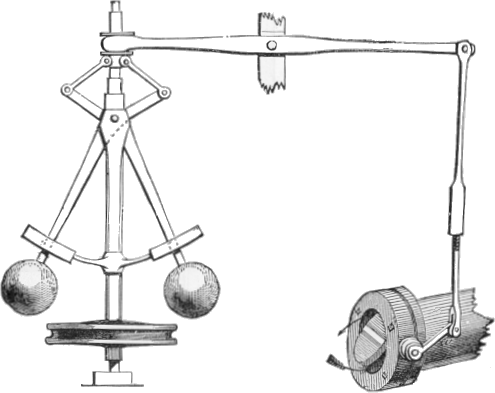
\includegraphics[width=8cm]{images/centrifugal_governor.png}
	\end{center}
	\supercaption{Le régulateur à boules, mécanisme provenant des moulins à vent et intégré aux moteurs à vapeur par James Watt.}{Dessin \pd \wcfile{Centrifugal_governor.png}{par R. Routledge (1900)}}
	\end{figure}

	Le jeune laborantin, qui porte le nom de \wf{James Watt}, trouve la fortune en s’associant avec un fabricant de canons expert en chaudronnerie, Matthew \mbox{Boulton}. La suite est sans équivoque : \textit{Boulton \& Watt} s’arrogeront une part énorme du marché naissant des machines thermiques.

	Leur succès, hélas, viendra bien moins des innovations technologiques apportées que des procès retentissants menés pour les monétiser. Car les deux partenaires excellent dans le relationnel politique et surtout dans l’univers particulier des brevets et des \textit{royalties} qui en découlent. Les deux Écossais à haut-de-forme touchent, par exemple, un pourcentage sur les économies de charbon engendrées par les machines qu’ils vendent à travers le pays. Et il faudra près d’une quinzaine d’années pour que s’ouvre enfin à tous la possibilité légale, au Royaume-Uni, d’utiliser la «~puissance expansive de la vapeur~», procédé sournoisement breveté par les deux associés !

	Quoi qu’il en soit, la \textit{Conférence générale des poids et mesures} attribua à la puissance l’unité \si{watt} dans la convention \textsc{si} en 1960. Elle détrôna alors le \emph{cheval-vapeur} (\textit{horsepower})… introduit par ledit James près d’un siècle plus tôt, pour comparer ses machines aux chevaux de trait qu’elles remplaçaient.
	\begin{IEEEeqnarray*}{rCl}
		\SI{1}{\cheval}_\text{impérial} 	& \equiv & \SI{33 000}{\foot\lbf\per\minute}\\
													& = & \SI{745.6999}{\watt}
	\end{IEEEeqnarray*}
	
\atendofhistorysection
